\documentclass{ltjbook}
\usepackage{docmute} 
\usepackage{../../myStyle} 

\begin{document}

\chapter{回帰分析の最尤推定}
\label{m24_maximum_likelihood}
前回は確率分布関数に含まれる変数の中で，パラメータの方が未知であると考えた尤度関数として捉え，尤度が最大になるようにパラメータの値を推定する\textbf{最尤推定法}について学びました。

今回はこれを，線形モデルに適用するお話です。線形モデルについては前期から今まで，折に触れては説明してきました。まず第\ref{m09_Regression}講で回帰分析に触れ，続いて重回帰分析(第\ref{m10_MultipleRegression}講)，それから要因計画へと展開してきたわけです。後期に入って推測統計学の話になり，要因計画と仮説検定の合体技，\keytermL{分散分析}{ぶんさんぶんせき}の話になりましたが，そこでの推定方法は\keytermL{モーメント法}{もーめんとほう}，すなわち\keytermL{標本平均}{ひょうほんへいきん}や\keytermL{不偏分散}{ふへんぶんさん}を使ってのものでした。\keytermL{平方和}{へいほうわ}を\keytermL{自由度}{じゆうど}で割って，\keytermL{平均平方}{へいきんへいほう}を出し，その比が\keytermL{F分布}{Fぶんぷ}に従う，という考え方は，平均や分散から母数を考えようという発想と同じものだと言えます。

それに対して，前回は尤度から母数を考えようという発想でした。推定値は同じになるのですが，考え方が違っていることに注意して，線形モデルの最尤推定について考えていきます。

\section{回帰分析と誤差分布}
改めて線形モデル，とくに\keytermL{単回帰分析}{たんかいきぶんせき}のモデルを復習しておきましょう。

データの組，$x_i,y_i$があった時に，変数$x$をつかって$y$を予測する，線形モデルを当てはめるということを考えるのでした。線形モデルは最も単純な一次式で，
\[\hat{y}_i = b_0 + b_1 x_i \]
とし，予測値$\hat{y}$に誤差$e$がついて実現値$y$が得られると考えて，
\[ y_i= b_0 + b_1 x_i + e_i  \]
とするのでした。第\ref{m08_CorrelationCausation}講でやった\keytermL{最小二乗法}{さいしょうにじょうほう}は，この式をデータに当てはめ，データの中で誤差が一番小さくなるように切片を求める，という方法だったことを思い出してください。あくまでも手元のデータの話しかしていませんでしたが，これに推測統計学のエッセンス，つまり手元のデータは標本に過ぎず，母集団の中でどうか，ということを考えたいと思います。

ところで，この時も仮定として誤差の分布に\keytermL{正規分布}{せいきぶんぷ}を仮定していましたね。誤差はさまざまな未知なる要因の積み重ねですから，数字を増やす方向に加わるのか，減らす方向に加わるのかは分かりません。それでも極端に大きな誤差というのは出にくく，平均周りの誤差が出やすいと考えるなら，単峰で左右対称のベルカーブのような形になるはずです。また，今回ここで考えているのは\keytermL{偶然誤差}{ぐうぜんごさ}ですから\footnote{これに対して\keytermL{系統誤差}{けいとうごさ}というのがありました。システマチックな誤差，という意味で，常に定数が加わるようなイメージです。体重計などの秤で何も測っていない時にメモリがずれているようなものですから，今回のケースではその補正は触れません。測定する際に気をつけるべきことで，気をつけてもなくならないのが偶然誤差です。}，その平均はゼロだと考えられます。ですから，$e_i = y_i - \hat{y}_i$をデータ全体で最小にするようにモデルをフィッティングするのでした。ここまでは前期の復習になります。

\section{確率モデル}
この線形モデルを確率モデルと考えて，最尤推定したい，というのがここでの狙いです。前期の最後，第\ref{m14_design3}講，セクション\ref{thinkWithDistribution}，Pp.\pageref{thinkWithDistribution}のあたりを思い出していただきたいところですが，大事なことなのでもう一度説明しておきましょう。

\keytermL{最尤推定}{さいゆうすいてい}をするためには，この回帰分析の式を確率モデルで表現しなければなりません。先ほどのモデル式の中に出てくる記号のなかで，確率的に変わるのは何かと言われれば，誤差$e$です。
そしてこれは，正規分布に従うだろうと考えるのが自然なのでした。式で書くと，
\[ e_i \sim N(0,\sigma) \]
ということになります。ここで誤差の平均が0である，ということを再確認してください。また，平均は0ですが，誤差は一定の幅で散らばって出てきますので，これを標準偏差$\sigma$で表しています。

さて，誤差が確率的に求まることがわかりましたが，$x$と$\hat{y}$の関係は確率的ではありません。切片や傾きは未知数ですが(母集団での切片と傾きのことになるので$\beta_0,\beta_1$と表記しますが)，これがわかりさえすれば$\hat{y}_i$と$x_i$の関係は確定的です。つまり，「確率分布に従う」を表す$\sim$という記号ではなく，「左辺はこのようになって\textbf{いる}」ということを記述するために，$=$を使って書くことができます。
\[ \hat{y}_i = \beta_0 + \beta_1 x_i \]
これが線形モデルです。誤差に邪魔されることがない，理想的な予測値$\hat{y}$は，$x_i$の一次関数の形で記述できる，ということです。実際のデータ$y_i$は$\hat{y}$に誤差がついて出てくるものですから，
\[ y_i = \hat{y}_i + e_i  \]
と書くことができます。

さて，これらを組み合わせていきましょう。最後の式から$\hat{y}$を消去する(線形モデルで代入する)と，
\[ y_i =  \beta_0 + \beta_1 x_i+ e_i \]
ということになります。ここで$ \beta_0 + \beta_1 x_i$のところは確率的に変わるものではない，ということを思い出してください。

\[
	y_i =
	\tcboxmath[
		enhanced,         % これは必須
		frame hidden,     % 枠を消す. これも enhanced 必須
		colback=cyan!10,
		overlay={
				\node[below,blue] at (frame.south) {確率的でないところ};
			}
	]{
		\beta_0 \quad +\quad \beta_1 x_i
	}
	+
	\tcboxmath[
		enhanced,         % これは必須
		frame hidden,     % 枠を消す. これも enhanced 必須
		colback=red!10,
		overlay={
				\node[below,red] at (frame.south) {確率的};
			}
	]{
		e_i
	}
\]

\vspace{0.5cm}
誤差$e_i$は平均0を中心に確率的に散らばりますが，その前のところは確率的ではありませんので，これを組み合わせた式全体としては，最後に確率的な散らばりがひっついているような形になります。数式ではありませんが，イメージでいうとこんな感じ。
\begin{center}
	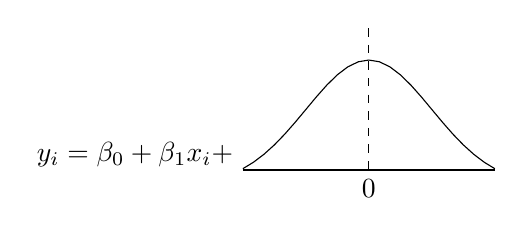
\begin{tikzpicture}[xscale = 0.8, yscale = 4]
		\coordinate (A) at (-2,0);
		\draw (A) node[left] {$y_i = \beta_0 + \beta_1 x_i + $};
		\draw [domain=-2:2] plot(\x, {exp((-(\x)^2)/2)/(sqrt(2*pi))-0.1});
		\draw [dashed] (0,0.4)--(0,-0.05);
		\draw (-2,-0.05)--(2,-0.05);
		\node (zero) at (0,-0.05)[below]{$0$};
	\end{tikzpicture}
\end{center}

さて，この「確率的でないところ」が確率分布の中に入り込むとしたら，誤差$e_i$の平均値を一定の量，$\beta_0 + \beta_1 x_i$分だけ動かすことになります。
回帰直線が表しているのは，誤差のない予測の線でもあります。実際のデータはそれに誤差が伴って生じます。確率モデルになった線形モデルは，図\ref{fig::24_01}のようなイメージで考えるといいかもしれません。
\begin{figure}[ht]
	\centering
	\includegraphics[keepaspectratio,width=0.8\linewidth]{../images/24_ML/Rplot24_06.png}
	\caption{予測直線にまとわりつく誤差}
	\label{fig::24_01}
\end{figure}

ここで正規分布がもつ2つのパラメータ，$\mu$と$\sigma$は，それぞれ\textbf{位置}と\textbf{幅}を表しているわけですが，確率的でないところはこの位置をズラすような作用をすることになります。

大事なところなので，もう一度式で確認しながら説明します。まず今回のモデルに含まれる情報は次のとおりです。
\begin{eqnarray}
	\hat{y}_i = \beta_0 + \beta_1 x_i \label{eq24_01}\\
	y_i = \hat{y}_i + e_i \label{eq24_02}\\
	e_i \sim N(0,\sigma)\label{eq24_03}
\end{eqnarray}
ここで式\ref{eq24_01}と\ref{eq24_02}を合わせて，
\begin{equation}
	\begin{array}{ccc}
		y_i & =    & \beta_0 + \beta_1 x_i +e_i \\
		e_i & \sim & N(0,\sigma)
	\end{array}
	\label{eq24_04}
\end{equation}
とします。ここで$e_i$の中心は$0$で，それに$\beta_0 + \beta_1 x_i$が加わるのですから，
\[ y_i \sim N(\beta_0 + \beta_1 x_i, \sigma) \]
ということになります。

あるいは，式\ref{eq24_02}と\ref{eq24_03}から先に，
\begin{eqnarray}
	\hat{y}_i &=& \beta_0 + \beta_1 x_i \label{eq24_05}\\
	y_i &\sim& N(\hat{y}_i,\sigma) \label{eq24_06}
\end{eqnarray}
と考えて，この式\ref{eq24_06}の$\hat{y}_i$に式\ref{eq24_05}を代入しても，
\[ y_i \sim N(\beta_0 + \beta_1x_i, \sigma) \]
が得られます。どちらのルートでも結構ですから，自分のわかりやすい方で理解してください。一覧の流れを図\ref{m24_two_way_root}にまとめてみました。
\begin{figure}[ht]
	\centering
	\begin{tikzpicture}
		\coordinate (A) at (1,1);
		\coordinate (B) at (2,2);
		\coordinate (C) at (5,2);
		\coordinate (D) at (7,1);
		\coordinate (E) at (1,3);
		\coordinate (F) at (7,3);
		\coordinate (G) at (1,5);
		\coordinate (H) at (7,5);
		\coordinate (I) at (1,7);
		\coordinate (J) at (2.5,6.5);
		\coordinate (K) at (5,6.5);
		\coordinate (L) at (7,7);
		\draw[->] (B)--(C);
		\draw[->] (G)--(E);
		\draw[->] (H)--(F);
		\draw[->] (J)--(K);
		\node (I1) at (0.3,6.5) {$\hat{y}_i  = \beta_0 + \beta_1x_i \ldots$(1)};
		\node (I2) at (0.54,6)  {${y}_i  = \hat{y}_i + e_i \ldots$(2)};
		\node (I3) at (0.5,5.5)  {$e_i \sim N(0,\sigma) \ldots$(3)};
		\node (L1) at (7,6)  {$e_i \sim N(0,\sigma)$};
		\node (L2) at (7,6.5) {${y}_i  = \beta_0 + \beta_1x_i + e_i$};
		\node (A1) at (0.5,2.5) {$\hat{y}_i  = \beta_0 + \beta_1x_i$};
		\node (A2) at (0.5,2) {$y_i \sim N(\hat{y}_i,\sigma)$};
		\node (D1) at (7,2) {$y_i \sim N(\beta_0 + \beta_1 x_i,\sigma)$};
		\node (P1) at (3.5,6.5)[above] {(2)に(1)を代入};
		\node (P2) at (1,4)[left] {(2)に(3)を代入};
		\node (P3) at (7,4)[right] {};
		\node (P4) at (3.5,2)[below] {};
	\end{tikzpicture}
	\caption{確率モデルと予測モデルの合体}
	\label{m24_two_way_root}
\end{figure}


これが回帰分析の\keytermL{確率モデル}{かくりつもでる}になります。
ポイントは，確率分布の位置を表すパラメータに，数式で表現された\textbf{構造}を書き込んだところにあります。狭義の\textbf{モデリング}とは，確率分布のパラメータに構造を与えるもの，ということができるでしょう。
発展的な話題になりますが，正規分布に限らず\keytermL{ベルヌーイ分布}{べるぬーいぶんぷ}や\keytermL{二項分布}{にこうぶんぷ}，\keytermL{ポアソン分布}{ぽあそんぶんぷ}などのパラメータを数式で表現したモデルを考えることもできます。正規分布以外の確率分布でパラメータに線形モデルを与えたものを\keyterm{一般化線形モデル}{いっぱんかせんけいもでる}{Generalized Linear Model}と呼びます\footnote{\keyterm{一般線形モデル}{いっぱんせんけいもでる}{General Linear Model}($\to$セクション\ref{GeneralLinearModel},Pp.\pageref{GeneralLinearModel})と混同しないように注意してください。}。一般化線形モデルになると，比率や度数などより広い範囲のデータを扱う分析ができるようになります\footnote{本学では二年次選択科目のデータ解析応用で扱います。興味がある人，履修をお待ちしています。}。

\section{確率モデルの最尤推定}

このようにして確率モデルを書くことができれば，あとはこれにしたがって「データがこの確率モデルから出てくる尤もらしさが最も高くなるように，未知パラメータを推定すれば良いということになります。
改めて確認ですが，今回のモデル$y_i \sim N(\beta_0 + \beta_1x_i, \sigma)$において未知な数字は$\beta_0,\beta_1,\sigma$の3つになります。


正規分布の式をちゃんと書くと，$x$という値が出てくる確率密度は
\[ p(x) = \frac{1}{\sqrt{2\pi \sigma^2}}exp\left( - \frac{(x-\mu)^2}{2\sigma^2}\right)\]
となります。この平均$\mu$のところに$\beta_0 + \beta_1 x_i$という数式を入れることになります。

すでに入り組んだ形をしているので，イメージしづらいところがあるかもしれませんが，あるデータ$y_i$が得られる確率密度は
\[ p(y_i) = \frac{1}{\sqrt{2\pi \sigma^2}}exp\left( -\frac{(y_i-\mu)^2}{2\sigma^2}\right)\]
ですから，$\mu=\hat{y_i} = \beta_0 + \beta_1 x_i$を代入して
\[ p(y_i) = \frac{1}{\sqrt{2\pi \sigma^2}}exp\left( -\frac{(y_i-\beta_0 - \beta_1 x_i)^2}{2\sigma^2}\right)\]
となります。

データは$i = 1,2,\cdots,N$とあり，それらが同じ母集団から独立に得られている，と考えます(i.i.d.)。つまり手元に同時にこれらのデータが出揃うときの尤度$L$は，上記の確率密度($p(y_i)$)を全部掛け合わせたもの\footnote{コインが表，表，裏，と出たら$\theta \times \theta \times (1-\theta)$と書けたことを思い出して！}，と考えることができますね。
$i$を$1$から$n$まで足し合わせることを総和する，といって$x_1+x_2+\cdots+x_N=\sum_{i=1}^N x_i$と表しますが，同様にすべて掛け合わせる総積は，
\[ x_1 \times x_2 \times \cdots x_N = \prod_{i=1}^N x_i \]
と書きます。ここでの記号$\prod$は\ruby{総積}{プロダクト}と言いますが，これを使って尤度$L(Y_i)$を表現すると，次のようになります。

\[ L(y_i | \beta_0,\beta_1,\sigma) = \prod_{i=1}^N \frac{1}{\sqrt{2\pi \sigma^2}}exp\left(- \frac{(y_i-\beta_0 - \beta_1 x_i)^2}{2\sigma^2}\right)\]

ここで$L(y_i | \beta_0,\beta_1,\sigma) $という書き方の，$\mid$は何かというと，この縦線の右側にある$\beta_0,\beta_1,\sigma$が与えられた場合の，という条件付き確率の書き方を借りた\keyterm{尤度}{ゆうど}{Likelihood}を表しています。

さてこれは確率(密度)の掛け算になりますから，すごく小さな数字になって実際の計算は大変です。そこで前回習ったように，尤度そのものではなく\keyterm{対数尤度}{たいすうゆうど}{log-likelihood}をとって，その最大値を求めるということにしたいと思います。対数をとると掛け算は足し算に変わりますから，$\prod \to \sum$に記号が変わりまして，対数尤度の関数は次のようになります。


非常に面倒な形をしていますね！しかもこれは$\beta_0,\beta_1,\sigma$という3つの変数が同時に関わりますから，連立微分方程式を解くことになります。

ここからは少しテクい話になりますが，この式を展開していきましょう。$\frac{1}{\sqrt{2\pi\sigma^2}}=(2\pi\sigma^2)^{-1/2}$であることに注意して対数尤度を書き直すと，

\begin{align*}
\log L &= \log\prod_{i=1}^n (2\pi\sigma^2)^{-1/2}\exp\left(-\frac{(y_i-(\beta_0+\beta_1x_i))^2}{2\sigma^2}\right) \\
&= \sum_{i=1}^n \log\left[(2\pi\sigma^2)^{-1/2}\exp\left(-\frac{(y_i-(\beta_0+\beta_1x_i))^2}{2\sigma^2}\right)\right] \\
&= \sum_{i=1}^n \left[\log(2\pi\sigma^2)^{-1/2} + \log\exp\left(-\frac{(y_i-(\beta_0+\beta_1x_i))^2}{2\sigma^2}\right)\right] \\
&= \sum_{i=1}^n \left[-\frac{1}{2}\log(2\pi\sigma^2) - \frac{(y_i-(\beta_0+\beta_1x_i))^2}{2\sigma^2}\right]\\
&= \sum_{i=1}^n \left[-\frac{1}{2}\log(2\pi) - \frac{1}{2}\log(\sigma^2) - \frac{(y_i-(\beta_0+\beta_1x_i))^2}{2\sigma^2}\right]\\
&= \frac{n}{2} \log(2\pi) - \frac{n}{2} \log(\sigma^2) - \frac{1}{2\sigma^2} \sum_{i=1}^{n} (y_i-(\beta_0+\beta_1x_i))^2
\end{align*}

こうしてみると，$\frac{n}{2} \log(2\pi)$は定数ですし，$\frac{n}{2} \log(\sigma^2) $は推定すべきパラメータ$\sigma^2$で，データによって変わるところではありません。
第3項の$\sum_{i=1}^{n} (y_i-(\beta_0+\beta_1x_i))^2$がデータによって変わるところで，これを最小化することを考える必要がありますが，これは最小二乗法で考えるべきポイントと同じですね。ですから，この最尤推定の結果得られる$\beta_0,\beta_1$の値は，\underline{最小二乗法の結果と一致}します。

もちろんこの面倒な計算は，Rがやってくれますから私たちはなんの心配もする必要はありません。
ですから，実質的にはただの回帰分析をすれば良いのです。

\subsection{実践例}
数字としてはなんら変わるところはないのですが，復習も兼ねて第\ref{m09_Regression}講でやった回帰分析をもう一度見てみましょう。
回帰分析の関数は\verb|lm|という関数名で，Rがデフォルトで持っている関数なのでした。実はこの関数，最尤推定値を返す関数だったのです。
そのときは\keytermL{最小二乗法}{さいしょうにじょうほう}の説明しかしていなかったのですが，関数の使い勝手のこともあって，最尤推定する関数でご紹介しておりました。
本当の意味で，最小二乗法のアルゴリズムで回帰分析をするときは\verb|lsfit|関数というものを使います。

使用例をコード\ref{code:24_01}に示しました。ここでは野球選手のデータを使って，身長から体重を予測するというモデルを実行しています\footnote{第\ref{m11_MRonR}講と同じ分析結果です。}。
\begin{lstlisting}[language=c++,label={code:24_01},caption={二つの推定法の比較}]
# 最小二乗法の推定
result.LS <- lsfit(x = batter$height, y = batter$weight)
result.LS$coefficients
# 最尤推定
result.LM <- lm(weight ~ height, data = batter)
result.LM
\end{lstlisting}
結果は出力\ref{RS:out24_01}のようになります。
\begin{Rscreen}{比較した結果}{out24_01}
	\begin{verbatim}
> # 最小二乗法の推定
> result.LS <- lsfit(x = batter$height, y = batter$weight)
> result.LS$coefficients
  Intercept           X 
-124.917552    1.166698 
> # 最尤推定
> result.LM <- lm(weight ~ height, data = batter)
> summary(result.LM)

Call:
lm(formula = weight ~ height, data = batter)

Residuals:
     Min       1Q   Median       3Q      Max 
-20.9217  -4.9213  -0.4214   4.0783  28.9118 

Coefficients:
              Estimate Std. Error t value Pr(>|t|)    
(Intercept) -124.91755   13.89317  -8.991   <2e-16 ***
height         1.16670    0.07746  15.063   <2e-16 ***
---
Signif. codes:  0 ‘***’ 0.001 ‘**’ 0.01 ‘*’ 0.05 ‘.’ 0.1 ‘ ’ 1

Residual standard error: 7.435 on 327 degrees of freedom
Multiple R-squared:  0.4096,	Adjusted R-squared:  0.4078 
F-statistic: 226.9 on 1 and 327 DF,  p-value: < 2.2e-16
    \end{verbatim}
\end{Rscreen}

これを見ると明らかなように，どちらの方法でやっても同じ推定値(切片$\beta_0=-124.918$，傾き$\beta_1=1.167$)になっていますね。また少し余談ではありますが，最尤推定した結果の最終行を見ると，$F$統計量が自由度$F(1,327)=226.9$とあり，この$p$値も計算されています。ここで線形モデルと要因計画・帰無仮説検定も関連があることがわかります\footnote{ここでは切片以外のすべての説明変数(今回の例では単回帰なので説明変数は一つですが)の傾きが0である，という帰無仮説にたいして検定が行われています。}。

方法が違っても推定値が同じ，というのは前回もお話ししたように，同じ母数を推定しているわけですからむしろ当然の結果です。1つの山の頂上に達するのに，複数のルートがあってもゴールは同じ，ということです。
違う点があるとすれば，最尤推定の場合は誤差の標準偏差$\sigma$も推定されているというところでしょうか。結果に$\sigma=...$という記載はありませんが，よく見ると\verb|Residuals|のところに残差$e$の最小値，最大値，四分位偏差，中央値などが示されており，誤差が分布するものと考えられていることがわかります。

今回は説明変数が1つの単回帰分析でしたが，説明変数の数が増えた\keyterm{重回帰分析}{じゅうかいきぶんせき}{Multiple Regression Analysis}でも同じで，\verb|lm|関数はデータが正規分布から得られたものとした上で，尤度を最大にする推定値を返してくれます。

Rで回帰分析をしたついでに，この結果をplot関数にいれてみましょう。
\begin{lstlisting}[language=c++,label={code:24_02},caption={回帰分析の結果オブジェクトをプロットに入れる}]
	par(mfrow = c(2, 2)) # 2x2の配置にする
	plot(result.LM)	
\end{lstlisting}

4つの図が表示されますが，ここでは$2\times 2$の配置にしています。出力されるのは図\ref{fig::24_02}のようになります。
\begin{figure}[ht]
	\centering
	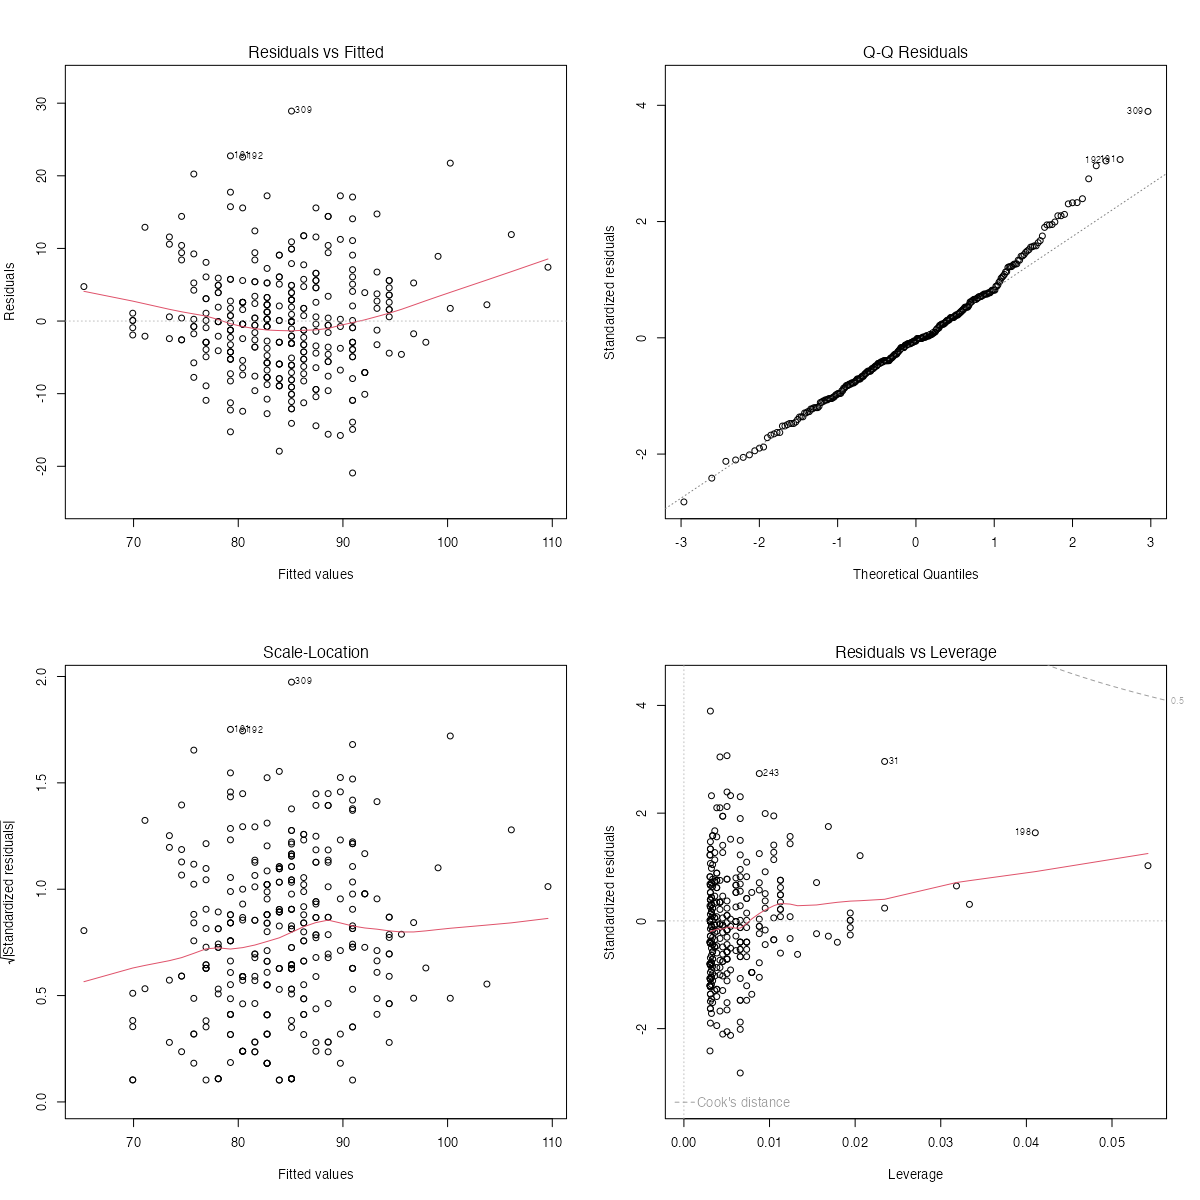
\includegraphics[keepaspectratio,width=0.8\linewidth]{../images/24_ML/Rplot_regression.png}
	\caption{回帰分析の結果をプロットすると4枚の図が出てくる}
	\label{fig::24_02}
\end{figure}

最初の図(図\ref{fig::24_02}左上)は，残差と予測値の散布図です。回帰分析において，残差$e_i$と予測値$\hat{y}_i$の相関は理論的にゼロになります。実践上そのようになっているかを確認するための図が表示されています。今回の散布図をみると，一定の関係はなさそう(緩やかなU字で，特定の関係があるように思えない)ですね。残差は規則性を持たず，均一に散らばっているはずです。この図を見てそれを確認しましょう。

第二の図(図\ref{fig::24_02}右上)は\keyterm{Q-Qプロット}{Q-Qぷろっと}{Q-Q plot}と呼ばれるものです。Q-Qプロットとは一般的に，データが仮定された確率分布に従っているかどうかを表示するためのもので，今回は横軸に正規分布の理論点を，縦軸に残差をプロットしています。理論通りの分布をしていると，左下から右上への45度線上にプロットされていくはずで，このラインから外れるのは理論分布から外れていることになります。今回は右の方，大きな値のところで少し歪みが生じていますが，ほとんどの点がライン上に載っていますので，まあ正規分布していたと考えられるでしょう。

第三の図(図\ref{fig::24_02}左下)は残差標準偏差と予測値のプロット，第四の図(図\ref{fig::24_02}右下)は残差とレバレッジの散布図です。レバレッジとは，各データ点がモデルに与える影響の大きさの指標です。これらも残差の分布が均一であるか，外れ値がないか，というところを検証するためのものです。

これらの図をみて残差が正規分布という仮定に従っているか，ということを確認することが重要です。こうした\keyterm{残差診断}{ざんさしんだん}{Residual Diagnostics}は，モデルの適合性や家庭の妥当性を評価しておくことが重要です。最尤法は確率モデルなのですから。

さて，こうしてみてくると，最小二乗法と最尤法，結局答えが同じになるのに，なぜこんな回りくどい話をするのかと思うかもしれません。
大事なのは線形モデルが確率モデルになったというところで，確率モデルになることで適用できる範囲が広がるから，というのが1つの答えです。
ところがもう1つ大事なことがあるのです。それは次回以降，第三の母数推定法である\keyterm{ベイズ法}{べいずほう}{Bayesian estimation method}に関係します。実はこの第三の方法も確率モデルを使ったものなのですが，詳しくは次回の講釈で。

\section{課題}
\paragraph{回帰分析の結果を読み取る}出力\ref{RS:out24_01}の読み取り方について，正しい記述をすべて選んでください。
\begin{itemize}
	\item 回帰係数が$1.166$である確率は$p<0.05$なので，滅多に得られる数字ではないから統計的に意味がない。
	\item 回帰係数の有意性検定が示しているのは，傾きが0であるという帰無仮説のもとで今回の係数$1.166$が得られる確率が小さい($p<0.05$)ということだから，統計的に意味がある。
	\item 今回のデータから考えると，回帰係数を$1.166$としたときに尤度が最も高くなる。
	\item 今回のデータから考えると，回帰係数を$1.166$としたときに残差の総量(二乗和)が最も小さくなる。
	\item 今回のデータから考えると，回帰係数が$1.166$となる確率は95\%以上である。
\end{itemize}
\end{document}
